\documentclass[all_sessions.tex]{subfiles}

\begin{document}

\notestitle{Session 2}{Exact Diagonalization of the Heisenberg Spin Chain}%
  {quantum\_magnetism.ipynb}{Session 1 (second quantization and the superexchange derivation of the
  Heisenberg model)}

\section*{Contents and goals}
Last time we ended on a cautionary note: mean-field theory, built entirely out of product states,
cannot represent the true ground state of the Hubbard dimer, an entangled singlet that spontaneously
breaks nothing at all. Today we stop approximating. Instead of guessing a variational ansatz, we are
going to write down the many-body Heisenberg Hamiltonian that emerges from superexchange, represent it
as an honest matrix acting on the full $2^L$-dimensional many-body Hilbert space, and diagonalize it
exactly. Along the way we will learn to read a many-body spectrum: how the many-body gap tells us
whether a spin chain is gapped or gapless, how a field or a coupling constant can be dialed to drive
level crossings and even phase transitions, how symmetries let us block-diagonalize the Hamiltonian so
that ``exact'' does not immediately mean ``impossible,'' and how correlators, both static and
dynamical, let us extract order and excitations directly from the wave function. We will close by
asking whether the excitations of a quantum magnet admit their own single-particle description, in
terms of emergent fermionic quasiparticles called spinons. Everything here is numerically exact, no
product-state restriction anywhere, and that honesty comes at the price we will keep bumping into all
session: the Hilbert space grows as $2^L$, which is exactly the wall that motivates the tensor-network
methods we build starting in Session 4.

\section*{Learning outcomes}
By the end of this session, you should be able to:
\begin{itemize}[nosep]
  \item Build the Heisenberg Hamiltonian as an explicit matrix on the many-body product-state
    basis and diagonalize it exactly for a finite spin chain.
  \item Use the finite-size scaling of the many-body gap, power-law versus saturating, to tell a
    gapless spin chain from a gapped one.
  \item Exploit conserved quantum numbers, total spin and $S_{\mathrm{tot}}^z$, to
    block-diagonalize the Hamiltonian and explain level crossings and magnetization curves in a
    field.
  \item Compute static and dynamical spin correlators and connect them to an auxiliary-fermion
    (spinon) mean-field description of the excitations.
\end{itemize}

\section{From the Hubbard dimer to a genuine quantum magnet}
\label{sec:setup}
Let us start by reminding ourselves what a symmetry-broken classical magnet actually looks like at the
microscopic level, since it is the natural foil for what comes next. Take the simplest possible
magnetic Hamiltonian, an Ising coupling between two spins,
\begin{equation}
  \Ham_{\mathrm{Ising}} = J\, S_1^z S_2^z, \qquad J>0.
  \label{eq:isingdimer}
\end{equation}
There is no $S^x$ or $S^y$ anywhere, so you can just as well think of $S_i^z=\pm\tfrac12$ as a classical
Ising variable. Minimizing the energy is trivial: we want $S_1^z$ and $S_2^z$ to have opposite sign, and
there are exactly two ways to do that, $\ket{\up\dn}$ and $\ket{\dn\up}$. Both are legitimate ground
states, both break time-reversal symmetry (flipping every spin sends one into the other), and each one
individually has a finite, sharply defined local moment $\expval{S_i^z}=\pm\tfrac12$. This is a classical
magnet in miniature: a genuinely symmetry-broken state with a finite magnetization at every site.

Now let us restore the full quantum mechanics of the spin operators and couple all three components,
\begin{equation}
  \Ham_{\mathrm{Heis}} = J\, \vb S_1\cdot\vb S_2 = J\left(S_1^xS_2^x + S_1^yS_2^y + S_1^zS_2^z\right).
  \label{eq:heisdimer}
\end{equation}
This is exactly the superexchange Hamiltonian we derived last session from the strong-coupling limit of
the Hubbard dimer, with $J=4t^2/U>0$. We already know, from Session 1, that its exact ground state is the
singlet $\ket{\Psi_{\mathrm{singlet}}}=\tfrac{1}{\sqrt2}(\ket{\up\dn}-\ket{\dn\up})$: a single,
non-degenerate state, with $\expval{S_i^z}=0$ on every site, that cannot be written as any product state.
This is what we will from now on call a genuine \textbf{quantum magnet}: unlike the Ising ground states,
this state does not break time-reversal symmetry at all, and it is entangled in an essential way.
Our job today is simply to compute this kind of ground state honestly, for chains longer than two sites,
and to understand everything we can read off from it and from the excited states that sit above it.

\section{Exact diagonalization: basis, matrix, and a worked dimer}
\label{sec:ed}
Generalize Eq.~\eqref{eq:heisdimer} to a chain of $L$ spin-$\tfrac12$'s with nearest-neighbor exchange,
\begin{equation}
  \Ham_{\mathrm{Heis}} = J\sum_{i=1}^{L-1} \vb S_i\cdot\vb S_{i+1}, \qquad J>0
  \ \text{(antiferromagnetic).}
  \label{eq:heisenberg}
\end{equation}
Regardless of how complicated $J_{ij}$ ends up being on some lattice, solving this Hamiltonian exactly
always reduces to the same three-step recipe: pick a basis of the many-body Hilbert space, write $\Ham$
as a matrix in that basis, and diagonalize it. The natural basis is the set of all product states
$\ket{\sigma_1\sigma_2\cdots\sigma_L}$ with $\sigma_i\in\{\up,\dn\}$: two states for $L=1$, four for
$L=2$, eight for $L=3$, and in general $2^L$ states for $L$ sites. This is precisely the exponential
growth of the many-body Hilbert space we have already met once, in Session 1's discussion of the Hubbard
model; here it shows up again because a spin-$\tfrac12$ chain is nothing but a projected, single-occupied
corner of that same fermionic Hilbert space.

To build the matrix we need the matrix elements of $\vb S_i\cdot\vb S_j$, and it is most convenient to
split it into a diagonal and an off-diagonal piece using the raising and lowering operators
$S^\pm = S^x\pm iS^y$,
\begin{equation}
  \vb S_i\cdot\vb S_j = S_i^zS_j^z + \tfrac12\left(S_i^+S_j^- + S_i^-S_j^+\right).
  \label{eq:sdots}
\end{equation}
The first term is diagonal in our product basis: it just multiplies each basis state by $\pm\tfrac14$
depending on whether $\sigma_i,\sigma_j$ are parallel or antiparallel. The second term is the one that
actually moves us around the basis: $S_i^+S_j^-$ flips an antiparallel pair $\dn_i\up_j\to\up_i\dn_j$
and annihilates everything else, so it only ever connects basis states that differ by swapping one
$\up\dn$ pair on a bonded pair of sites. This is why the Heisenberg matrix, even though it lives in a
$2^L$-dimensional space, is \emph{sparse}: each row has at most $L-1$ off-diagonal entries, one per bond,
which is exactly the kind of structure that iterative solvers like Lanczos exploit to reach much bigger
$L$ than a naive dense diagonalization ever could.

\paragraph{Worked example: the dimer, twice over.} Let us see this explicitly for $L=2$. In the basis
$\{\ket{\up\up},\ket{\up\dn},\ket{\dn\up},\ket{\dn\dn}\}$, the stretched states $\ket{\up\up}$ and
$\ket{\dn\dn}$ have no partner to flip into, so $\Ham_{\mathrm{Heis}}\ket{\up\up}=\tfrac{J}{4}\ket{\up\up}$
and likewise for $\ket{\dn\dn}$. On the remaining two-dimensional subspace $\{\ket{\up\dn},\ket{\dn\up}\}$,
Eq.~\eqref{eq:sdots} gives the $2\times2$ block
\begin{equation}
  \Ham_{\mathrm{Heis}}\Big|_{\{\up\dn,\dn\up\}} = J\begin{pmatrix} -\tfrac14 & \tfrac12 \\[2pt]
    \tfrac12 & -\tfrac14 \end{pmatrix}
  \;\Longrightarrow\;
  E_\pm = J\left(-\tfrac14\pm\tfrac12\right), \qquad
  \ket{\pm} = \tfrac{1}{\sqrt2}\left(\ket{\up\dn}\pm\ket{\dn\up}\right).
  \label{eq:dimermatrix}
\end{equation}
So $E_-=-\tfrac34 J$ for the antisymmetric combination, exactly the singlet we already knew, and
$E_+=\tfrac14 J$ for the symmetric combination, degenerate with $\ket{\up\up}$ and $\ket{\dn\dn}$ at the
same energy $\tfrac{J}{4}$: together these three states form the \textbf{triplet}. Diagonalizing a
$4\times4$ matrix by hand already reproduces the full singlet/triplet structure.

There is a second, quicker way to get the same answer, and it is worth knowing because it generalizes.
Define the total spin $\vb S_{\mathrm{tot}} = \vb S_1+\vb S_2$, so that
$\vb S_{\mathrm{tot}}^2 = \vb S_1^2+\vb S_2^2+2\,\vb S_1\cdot\vb S_2$, and hence
\begin{equation}
  \Ham_{\mathrm{Heis}} = J\,\vb S_1\cdot\vb S_2
    = \frac{J}{2}\left[S_{\mathrm{tot}}(S_{\mathrm{tot}}+1) - \tfrac34 - \tfrac34\right],
  \label{eq:dimerspec}
\end{equation}
using $\vb S_i^2=\tfrac34$ for spin-$\tfrac12$. Since $\vb S_{\mathrm{tot}}^2$ has eigenvalues
$S_{\mathrm{tot}}(S_{\mathrm{tot}}+1)$ with $S_{\mathrm{tot}}=0$ or $1$ for two spin-$\tfrac12$'s,
Eq.~\eqref{eq:dimerspec} immediately gives $E(S_{\mathrm{tot}}=0)=-\tfrac34J$ and
$E(S_{\mathrm{tot}}=1)=\tfrac14J$, matching Eq.~\eqref{eq:dimermatrix} exactly. Notice, too, why the
notebook's ground-state energy happens to equal the sum of the separately computed Ising and XY ground
energies: on the two-dimensional subspace $\{\ket{\up\dn},\ket{\dn\up}\}$, the Ising piece $S_1^zS_2^z$ is
literally proportional to the identity, $-\tfrac14\mathbb{1}$, since \emph{both} basis states carry the
same $S_1^zS_2^z$ eigenvalue. Minimizing the sum of a constant and the XY block is the same as minimizing
each separately and adding, which is why the two energies happen to add up here. This is special to
$L=2$: for longer chains the Ising term is no longer a multiple of the identity on the subspace the XY
term mixes, and the two pieces generically no longer minimize on the same state.

\begin{notebook}
Open \texttt{quantum\_magnetism.ipynb} and work through the ``Basics'' block: ``Creating a
spin\_chain object,'' ``Creating a Hamiltonian,'' ``Computing the ground state energy,'' and
``Computing expectation values.'' Build the $L=2$ Heisenberg Hamiltonian directly from the spin
operators, diagonalize it, and check that you recover $E_{\mathrm{singlet}}=-\tfrac34J$ and
$E_{\mathrm{triplet}}=\tfrac14J$ numerically. Then replace $S^x$ by $S^y$ in the expectation-value cell
and think about why nothing changes.
\end{notebook}

\section{The many-body spectrum and the many-body gap}
\label{sec:gap}
Now let us stop looking at $L=2$ by hand and let the computer diagonalize Eq.~\eqref{eq:heisenberg} for
increasing $L$. The number of eigenvalues you get out is, of course, exactly the dimension of the
matrix, $2^L$: two for $L=2$, sixteen for $L=4$, sixty-four for $L=6$, and so on, growing exponentially
with system size, exactly like the basis itself. In practice, though, we almost never care about the
whole spectrum. Any real experiment at low temperature only probes the states closest to the ground
state, so from now on we will systematically focus on the bottom of the many-body spectrum: the ground
state $E_0$ and the handful of low-lying excited states just above it.

The single most useful number we can read off from this part of the spectrum is the \textbf{many-body
gap},
\begin{equation}
  \Delta(L) \equiv E_1(L) - E_0(L),
  \label{eq:manybodygap}
\end{equation}
the energy cost of the cheapest excitation above the ground state. For the uniform Heisenberg chain,
$\Delta(L)$ shrinks steadily as $L$ grows, and it does so following a power law rather than saturating
to a finite value: this is the hallmark of a \textbf{gapless} system, one whose excitations become
arbitrarily cheap in the thermodynamic limit. Where does this power law come from? Qualitatively, from
exactly the same free-fermion logic we will use in Section~\ref{sec:spinon}: replace each spin operator
by an auxiliary (Abrikosov) fermion $f_{i\sigma}$ and mean-field decouple the exchange term, and
$\Ham_{\mathrm{Heis}}$ turns into a free-fermion \textbf{spinon} Hamiltonian whose band is gapless, with
Fermi points at $k_F=\pm\pi/2$. The cheapest excitations are then particle-hole pairs created right at
those Fermi points, which disperse \emph{linearly} in momentum, and a linearly dispersing excitation on a
ring of $L$ sites is exactly a one-dimensional particle-in-a-box problem: its levels are spaced by
\begin{equation}
  \Delta(L) \;\sim\; \frac{\pi v_s}{L},
  \label{eq:gapscaling}
\end{equation}
with $v_s$ the velocity of the low-energy excitations, i.e.\ a genuine $1/L$ power law rather than a
finite gap. (Numerically, the finite-size data is well fit by $\Delta(L)\approx\pi^2J/(2L)$; pinning down
$v_s$ this precisely is a job for the exact Bethe-ansatz solution, not for mean-field theory, which gets
the qualitative power law right but not the precise coefficient.) Keep this ``particle in a box'' picture
in mind: we will meet it again, in a much more literal form, when we look at dynamical correlators in
Section~\ref{sec:dynamical}, and again when we build the explicit spinon band structure behind this
argument in Section~\ref{sec:spinon}.

\begin{notebook}
Section ``Many-body energies of the Heisenberg model.'' Diagonalize the uniform chain for
$L=2,4,6,8$ and plot the full spectrum each time: check that the number of eigenvalues really is
$2^L$. Then plot only $E_1(L)-E_0(L)$ and see the gap shrink with $L$; think about what the biggest
$L$ is that you could still store the full spectrum for on your own machine.
\end{notebook}

\section{The XXZ model: from classical order to quantum entanglement}
\label{sec:xxz}
Section~\ref{sec:setup} presented the Ising model and the Heisenberg model as two separate
Hamiltonians, but it is much more illuminating to see them as the two endpoints of a single family. Take
\begin{equation}
  \Ham_{\mathrm{XXZ}} = \sum_i \left[J_{xy}\left(S_i^xS_{i+1}^x + S_i^yS_{i+1}^y\right)
    + J_z\, S_i^zS_{i+1}^z\right], \qquad J_z\equiv 1 \text{ fixed},
  \label{eq:xxz}
\end{equation}
and dial $J_{xy}$ from $0$ to $1$. At $J_{xy}=0$ we are exactly back at the classical Ising model of
Eq.~\eqref{eq:isingdimer}, generalized to $L$ sites: in the thermodynamic limit its ground state is
doubly degenerate, the N\'eel-ordered $\ket{\up\dn\up\dn\cdots}$ and its time-reversed partner, each
carrying a finite, symmetry-broken staggered moment. At $J_{xy}=1$ we recover the isotropic Heisenberg
model of Eq.~\eqref{eq:heisenberg}, whose ground state, as we already know from the dimer, is unique and
carries no local moment at all: a purely quantum magnet. So $J_{xy}$ literally interpolates between a
classical, symmetry-broken magnet and a quantum, entangled one, and the natural question is: how does
the ground state actually get from one description to the other as we sweep $J_{xy}$?

\begin{figure}[H]
  \centering
  \begin{subfigure}[c]{0.46\textwidth}
    \centering
    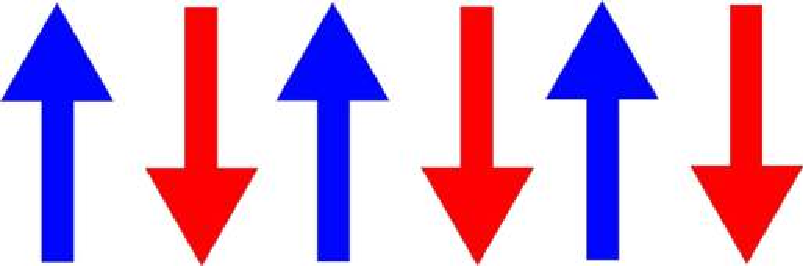
\includegraphics[width=\linewidth]{figures/quantum_magnetism/ising_gs_a.pdf}
    \caption{$\ket{\up\dn\up\dn\cdots}$}
  \end{subfigure}\hfill
  \begin{subfigure}[c]{0.46\textwidth}
    \centering
    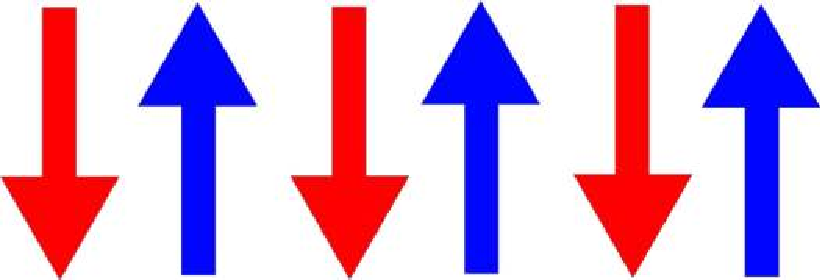
\includegraphics[width=\linewidth]{figures/quantum_magnetism/ising_gs_b.pdf}
    \caption{$\ket{\dn\up\dn\up\cdots}$}
  \end{subfigure}
  \caption{The two classical ground states of Eq.~\eqref{eq:xxz} at the Ising endpoint
    $J_{xy}=0$. Each is a product state with a definite $S^z$ on every site, each carries a
    finite staggered moment, and the two are exchanged by time reversal. In the thermodynamic
    limit they are exactly degenerate and the system picks one of them, which is what symmetry
    breaking means here. On a finite chain they are instead split by a tiny amount, and watching
    that splitting grow as $J_{xy}\to1$ is how the crossover to the unique, entangled Heisenberg
    ground state shows up in the spectrum.}
  \label{fig:neel-pair}
\end{figure}

The finite-size spectrum answers this beautifully. At small $J_{xy}$, the two classical N\'eel states are
not exactly degenerate on a finite chain (only a genuinely infinite chain can spontaneously break a
symmetry), but they sit extremely close together, split by a tiny amount that we can literally watch on
the screen: this is the finite-size ghost of the classical double degeneracy. As we increase $J_{xy}$
toward $1$, this splitting grows continuously, and for any finite $L$ that growth eventually turns into a
finite, clearly non-degenerate gap once $J_{xy}$ gets close enough to $1$. What changes as we make $L$
bigger is exactly how close to $J_{xy}=1$ this crossover sits: for larger and larger chains, the two
low-lying states stay nearly degenerate over a longer and longer stretch of $J_{xy}$, and the crossover
sharpens toward the exact, thermodynamic-limit transition of the XXZ chain, which the Bethe-ansatz
solution places precisely at the isotropic, SU(2)-symmetric point $J_{xy}=J_z$. In other words: just by
watching how two eigenvalues in a finite-size spectrum move and split as we tune a coupling constant, we
can already diagnose a genuine quantum phase transition, well before we ever reach the thermodynamic
limit itself. This is a technique we will lean on again and again in the rest of the course.

\begin{notebook}
Section ``From classical to quantum magnetism.'' Plot the low-lying spectrum of
$\Ham_{\mathrm{XXZ}}$ as a function of $J_{xy}$ at fixed $L$: identify the near-degenerate pair at
small $J_{xy}$ and watch it split as $J_{xy}\to1$. Then increase $L$ and see how the splitting
crossover sharpens and moves, tracking the exact thermodynamic-limit transition at the isotropic
point.
\end{notebook}

\section{Good quantum numbers: total spin, the Zeeman field, and block-diagonalization}
\label{sec:quantumnumbers}
Section~\ref{sec:ed} used the identity $\vb S_1\cdot\vb S_2=\tfrac12[\vb S_{\mathrm{tot}}^2 - \vb
S_1^2-\vb S_2^2]$ as a shortcut for the dimer, but it is worth asking why it worked: it worked because
$\vb S_{\mathrm{tot}}^2$ and $S_{\mathrm{tot}}^z$ commute with $\Ham_{\mathrm{Heis}}$. This is not
special to two sites. Because Eq.~\eqref{eq:heisenberg} is built entirely out of dot products
$\vb S_i\cdot\vb S_j$, it is invariant under any global spin rotation, and Noether's theorem in its
operator form tells us immediately that the total spin $\vb S_{\mathrm{tot}}=\sum_i \vb S_i$ is
conserved for \emph{any} $L$ and any choice of exchange couplings $J_{ij}$:
\begin{equation}
  \left[\Ham_{\mathrm{Heis}},\, \vb S_{\mathrm{tot}}^2\right] = 0, \qquad
  \left[\Ham_{\mathrm{Heis}},\, S_{\mathrm{tot}}^z\right] = 0.
  \label{eq:conservation}
\end{equation}
So every eigenstate of $\Ham_{\mathrm{Heis}}$ can be labeled by a definite total spin $S$ and a definite
projection $m$, exactly the singlet ($S=0$) and triplet ($S=1$) labels we used for the dimer, now
promoted to good quantum numbers for a chain of any length.

\paragraph{The Zeeman field does not mix states.} Let us now add a uniform magnetic field,
\begin{equation}
  \Ham(B) = \Ham_{\mathrm{Heis}} - B\, S_{\mathrm{tot}}^z.
  \label{eq:zeeman}
\end{equation}
This term explicitly singles out the $z$-axis, so it breaks the full SU(2) spin-rotation symmetry down
to rotations about $z$ alone. But look closely at what it actually does to our two conserved quantities.
It trivially commutes with $S_{\mathrm{tot}}^z$, since it is built out of nothing else. And because
$[\vb S_{\mathrm{tot}}^2, S_{\mathrm{tot}}^z]=0$ is a completely general identity of angular momentum
algebra, $\Ham(B)$ \emph{also} commutes with $\vb S_{\mathrm{tot}}^2$. So both quantum numbers survive
even in the presence of the field: adding $B$ cannot mix any eigenstates of $\Ham_{\mathrm{Heis}}$ into
each other, it can only shift each one's energy by $-Bm$. This is exactly why the field-dependent
spectrum you see in the notebook is a set of perfectly straight lines rather than curves: each state
with a definite $m$ shifts linearly, $E(B)=E(0)-Bm$, and states only bend or avoid one another once you
add a term, like a transverse field, that fails to commute with $S_{\mathrm{tot}}^z$.

Applied to the dimer: the singlet has $m=0$ and stays completely flat, $E_{\mathrm{singlet}}(B)=-\tfrac34
J$. The triplet's three members split according to their own $m=-1,0,+1$: the $m=0$ member is also
completely flat, at $E=\tfrac14J$, while the $m=\pm1$ members disperse as $E=\tfrac14J\mp B$. Those are
precisely the two ``flat lines'' you can spot in the notebook's zero-field spectrum: they sit at
different energies, separated by exactly the many-body gap $\Delta=J$ of Eq.~\eqref{eq:manybodygap}, and
what distinguishes them is not $m$, which is $0$ for both, but the total spin $S$, $0$ for one and $1$
for the other.

\paragraph{Block-diagonalizing a long chain.} The real payoff of Eq.~\eqref{eq:conservation} is
computational. Since $S_{\mathrm{tot}}^z=\sum_i S_i^z$ is conserved, the full $2^L\times2^L$ Hamiltonian
never actually mixes basis states with different numbers of up spins: if $n_\up$ counts the up spins,
then $m=n_\up-L/2$ is fixed within each block, and $\Ham_{\mathrm{Heis}}$ is block-diagonal with blocks
of dimension
\begin{equation}
  \dim(m) = \binom{L}{L/2+m}.
  \label{eq:szsector}
\end{equation}
The largest block sits at $m=0$ (for even $L$), with $\dim(0)=\binom{L}{L/2}\sim 2^L/\sqrt{\pi L/2}$ by
Stirling's approximation: still exponential in $L$, but a factor $\sim\sqrt L$ smaller than the full
Hilbert space, and, crucially, diagonalizable completely independently of every other block. If the
chain is also periodic, translational invariance gives us a second conserved quantity, the total
momentum $k$, and combining Sz-sectors with momentum sectors shrinks the largest block by roughly
another factor of $L$. This combination, exploiting every available conserved quantity together with the
sparse-matrix Lanczos techniques of Section~\ref{sec:ed}, is exactly how a code like \texttt{dmrgpy}
manages to push exact diagonalization out to the $L\lesssim20$ spins we will be working with all
session; without it, $2^{20}\approx10^6$ would already be a serious dense-matrix computation, and $L=30$
would simply be out of reach.

\begin{figure}[H]
  \centering
  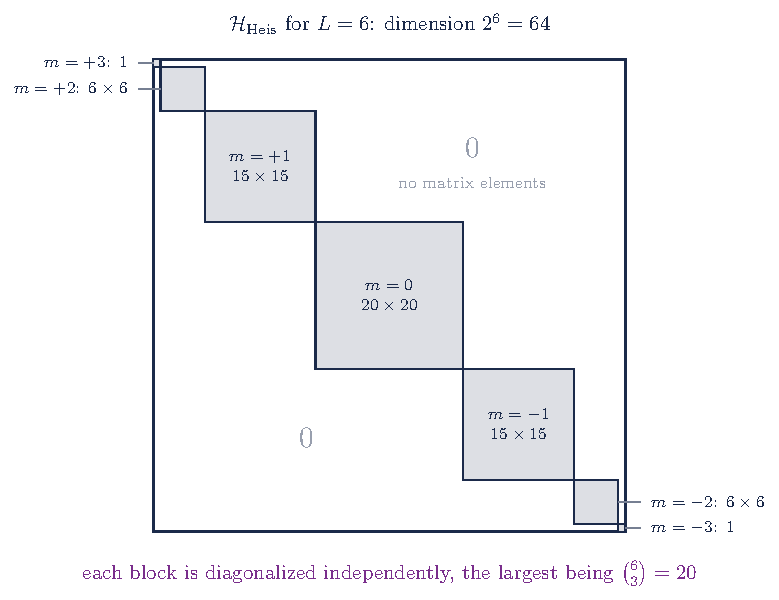
\includegraphics[width=0.72\textwidth]{figures/sz_blocks.pdf}
  \caption{Block structure of $\Ham_{\mathrm{Heis}}$ in the $S_{\mathrm{tot}}^z$ basis, drawn for
    $L=6$ with the blocks to scale. Because $S_{\mathrm{tot}}^z$ is conserved, the Hamiltonian
    never connects basis states with different numbers of up spins, so the $2^L\times2^L$ matrix
    falls apart into one block per magnetization sector, of dimension
    $\binom{L}{L/2+m}$ as in Eq.~\eqref{eq:szsector}, with nothing at all outside them. Each block
    is diagonalized completely independently of the others, and even the largest one, at $m=0$, is
    already smaller than the full space by a factor $\sim\sqrt L$.}
  \label{fig:sz-blocks}
\end{figure}

\begin{notebook}
Sections ``Energies of a Heisenberg model as a function of the external magnetic field'' and
``Quantum numbers in the Heisenberg model.'' Plot the dimer spectrum against $B$ and check the
linear, non-mixing evolution predicted by Eq.~\eqref{eq:zeeman}; identify which line is the singlet
and which is the $m=0$ triplet member, and confirm that they are exactly $\Delta=J$ apart at $B=0$.
Then think about what field-dependent term would bend the lines instead of keeping them straight.
\end{notebook}

\section{Level crossings and magnetization curves}
\label{sec:levelcrossings}
Equation~\eqref{eq:zeeman} does more than split levels: because different $m$-sectors disperse with
different slopes, they can cross, and a crossing at the very bottom of the spectrum is a genuine
\textbf{level crossing of the ground state}. For the dimer this is easy to pin down exactly: the
ground state is the singlet, at $-\tfrac34J$, until the $m=+1$ triplet branch $E=\tfrac14J-B$ drops below
it, which happens once
\begin{equation}
  \tfrac14J - B = -\tfrac34J \quad\Longrightarrow\quad B = J.
  \label{eq:crossingfield}
\end{equation}
Below $B=J$ the ground state is the singlet, with zero magnetization; above $B=J$ it is the fully
polarized triplet member $\ket{\up\up}$, with saturated magnetization $\expval{S_{\mathrm{tot}}^z}=1$.
This is the simplest possible example of a field-driven quantum phase transition: a single, sharp level
crossing between a sector with $S=0$ and a sector with $S=1$.

Longer chains show the same phenomenon, just repeated many times over. As $B$ grows from zero, the
ground state hops successively through sectors of increasing total spin, $S=0\to1\to2\to3\to\cdots$,
each hop showing up as an abrupt jump in the ground-state magnetization $\expval{S_{\mathrm{tot}}^z}$: a
magnetization staircase. Because bigger chains pack their low-lying $S$-sectors closer together in
energy, these crossings happen at progressively smaller fields as $L$ grows, and in the thermodynamic
limit the staircase smooths out into the continuous magnetization curve of an infinite antiferromagnetic
chain. Eventually, once $B$ exceeds roughly the bandwidth of the low-energy spectrum ($B\gtrsim zJ$, with
$z$ the coordination number; for a chain, $z=2$ and the saturation field is exactly $B_{\mathrm{sat}}=2J$),
the ground state saturates completely: every spin points along the field,
and this fully polarized state is in fact an \emph{exact} eigenstate of $\Ham_{\mathrm{Heis}}$ itself, a
rare case where the many-body ground state really is a simple product state, since there is nothing left
for the exchange term to do once every spin is already maximally aligned. Sweeping $B\to-B$ reproduces
the identical staircase with the opposite sign of magnetization, exactly the time-reversal partner of the
$B>0$ curve.

It is also worth looking directly at the excited states in a small field, before any level crossing has
happened. The ground state stays a total-$S=0$ singlet with zero magnetization on every site. The first
excited states, the $S=1$ triplet members, do carry a finite total magnetization, but that magnetization
is not localized anywhere: it is smeared out over the whole chain, one more signature that these are
genuinely delocalized many-body excitations rather than a single flipped spin sitting at one site.
Higher excited states repeat this pattern with different sign structures, several of them related to
each other by time reversal, and this whole family of spread-out, roughly particle-in-a-box-like
excitations is exactly what the dynamical correlator of Section~\ref{sec:dynamical} will let us resolve
in detail.

\begin{notebook}
Sections ``Level crossings in the Heisenberg model,'' ``Many-body wavefunctions in a magnetic
field,'' ``Level crossings as a function of the magnetic field,'' and ``Magnetization of moderately
large Heisenberg model.'' Confirm the dimer's crossing at $B=J$ from Eq.~\eqref{eq:crossingfield},
then move to $L=6$ and $L=10$ chains and track the full magnetization staircase, its saturation field,
and its mirror symmetry under $B\to-B$.
\end{notebook}

\section{Gapped versus gapless: the dimerized chain}
\label{sec:dimerization}
Section~\ref{sec:gap} told us the uniform Heisenberg chain is gapless, $\Delta(L)\to0$ as a power law.
Let us now build a chain that is not, by alternating the exchange coupling bond by bond,
\begin{equation}
  \Ham_{\mathrm{dimer}} = \sum_i J_i\, \vb S_i\cdot\vb S_{i+1}, \qquad
  J_i = J\left[1+(-1)^i\delta\right],
  \label{eq:dimerized}
\end{equation}
so odd and even bonds alternate between $J(1+\delta)$ and $J(1-\delta)$. At $\delta=0$ we recover the
uniform, gapless chain. At the opposite extreme $\delta\to1$, the weak bonds vanish entirely and the
chain falls apart into $L/2$ completely decoupled dimers, each one exactly the $L=2$ problem of
Section~\ref{sec:ed}: the exact ground state is simply a product of singlets, one per strong bond, and
the cheapest excitation is a single dimer flipping from its singlet into its triplet, costing exactly
$\Delta_\infty = J(1+\delta)$, the very same singlet-triplet gap we computed in
Eq.~\eqref{eq:dimermatrix}. Turning the weak bond back on perturbs this picture, letting the singlets
talk to each other and giving the triplet excitation some dispersion, but it does not close the gap: for
any finite $\delta$, no matter how small, the dimerized chain remains gapped, with a finite $\Delta_\infty$
that shrinks smoothly to zero only as $\delta\to0$.

This qualitative difference shows up very cleanly in how $\Delta(L)$ approaches its thermodynamic-limit
value. For the gapless uniform chain, we already saw the slow, power-law approach of
Eq.~\eqref{eq:gapscaling}: even $L\sim20$ is not enough to convince yourself the gap is really heading to
zero. For the dimerized chain, a finite gap sets its own length scale, the correlation length
$\xi\sim v_s/\Delta_\infty$, and finite-size corrections to the gap are suppressed exponentially,
$\Delta(L)-\Delta_\infty \sim e^{-L/\xi}$, rather than as a power law. That is why, numerically, a
dimerized chain's gap already looks converged by $L\sim12$--$14$, while the uniform chain's gap is still
visibly drifting at the same size: the presence or absence of a length scale $\xi$ is precisely what
separates fast, exponential finite-size convergence from slow, power-law convergence.

\begin{notebook}
Section ``Gap of a many-body spin chain.'' Compute $\Delta(L)$ for the uniform chain ($\delta=0$)
and for a dimerized chain ($\delta>0$), and compare how quickly each one saturates as you increase
$L$; check that the dimerized gap has essentially converged well before the uniform one has.
\end{notebook}

\section{Diagnosing the gap: impurities and non-local correlators}
\label{sec:diagnostics}
Comparing gaps at different $L$ works, but it needs several system sizes side by side. Is there a way
to diagnose gapped versus gapless behavior from a \emph{single} calculation? Yes: look at how the system
responds in space rather than how its energy responds in size.

\paragraph{A magnetic impurity.} Pin a small local field on one site, $\Ham\to\Ham_{\mathrm{Heis}} - h\,
S_{i_0}^z$, and measure the induced magnetization profile $\expval{S_j^z}$ as a function of distance
$r=|j-i_0|$ from the impurity. For the gapless uniform chain, this response decays \emph{algebraically},
$\expval{S_j^z}\sim r^{-1}$, the standard hallmark of critical, scale-free correlations in a
one-dimensional gapless system. For the gapped dimerized chain, the very same measurement decays
\emph{exponentially}, $\expval{S_j^z}\sim e^{-r/\xi}$, with the same correlation length $\xi$ that
controlled the finite-size convergence of the gap in Section~\ref{sec:dimerization}. So the way a
localized perturbation ``heals'' as you move away from it already tells you, from a single system size,
whether the underlying chain is gapped or gapless.

\paragraph{Non-local static correlators.} We can get exactly the same information without introducing
any impurity at all, by computing the connected two-point correlator
\begin{equation}
  C(i,j) = \expval{\vb S_i\cdot\vb S_j} - \expval{\vb S_i}\cdot\expval{\vb S_j}.
  \label{eq:correlator}
\end{equation}
In a genuine quantum magnet $\expval{\vb S_i}=0$ everywhere, so this reduces to the bare correlator
$\expval{\vb S_i\cdot\vb S_j}$; for a classical, product-state magnet, on the other hand, $C(i,j)$
vanishes identically, since a product state trivially factorizes the expectation value. So a nonzero
$C(i,j)$ is itself a direct signature of entanglement beyond any mean-field description, echoing exactly
the failure mode we uncovered for the Hubbard dimer in Session 1. Formally, this static correlator is
tied to the impurity response of the previous paragraph by linear response (a Kubo-formula argument):
the induced magnetization at $j$ from a small field at $i$ is, to leading order, proportional to
$C(i,j)$ itself. It is therefore no surprise that $C(i,j)$ shows exactly the same dichotomy: power-law
decay for the gapless chain, exponential decay, with a rate set by $\delta$, for the dimerized one. The
bigger the dimerization, the bigger the gap, and the faster $C(i,j)$ falls off, a clean, single-snapshot
diagnostic for how gapped a quantum magnet really is.

\begin{notebook}
Sections ``Magnetization of a Heisenberg model with a magnetic impurity,'' ``Magnetization of a
dimerized Heisenberg model with a magnetic impurity,'' and ``Non-local static correlators.'' Compare
the decay of the induced magnetization for the uniform and dimerized chains, then compute
Eq.~\eqref{eq:correlator} directly for several values of the dimerization and check that faster decay
tracks a bigger gap.
\end{notebook}

\section{Dynamical correlators, and a first look at spin-1}
\label{sec:dynamical}
So far we have only used static, equal-time expectation values. A \textbf{dynamical spin correlator}
carries strictly more information, because it resolves excitations by their energy as well as their
location. Define
\begin{equation}
  S(i,\omega) = \bra{0}S_i^z\,\delta(\omega - (\Ham-E_0))\,S_i^z\ket{0}.
  \label{eq:dyncorrdef}
\end{equation}
This looks abstract until we insert a resolution of the identity in the exact eigenbasis of $\Ham$,
$\mathbb{1}=\sum_n\ket{n}\bra{n}$, which turns Eq.~\eqref{eq:dyncorrdef} into the Lehmann representation
\begin{equation}
  S(i,\omega) = \sum_n \left|\bra{n}S_i^z\ket{0}\right|^2 \, \delta\!\left(\omega - (E_n-E_0)\right).
  \label{eq:lehmann}
\end{equation}
Read this as a spectroscopy experiment: it says that if you inject a spin flip at site $i$ with energy
$\omega$, you get a nonzero response exactly when there exists an eigenstate $\ket{n}$ at energy
$E_n=E_0+\omega$ that is actually connected to the ground state by a local spin flip, weighted by how big
that overlap $\bra{n}S_i^z\ket{0}$ is.

For the spin-$\tfrac12$ uniform chain, $S(i,\omega)$ shows a sequence of discrete peaks, spread out over
the whole chain, separated by gaps: exactly the particle-in-a-box quantization we anticipated in
Eq.~\eqref{eq:gapscaling}. As $L$ grows, these peaks soften toward lower $\omega$, tracking the shrinking
many-body gap of Section~\ref{sec:gap}, and more of them appear as the low-energy spectrum becomes
denser.

\paragraph{A first look at spin-1.} If we redo this same calculation for a spin-$1$ Heisenberg chain
instead of spin-$\tfrac12$, the profile of $S(i,\omega)$ looks qualitatively different. This is because
the two cases sit in genuinely different phases: the spin-$\tfrac12$ chain is gapless in the
thermodynamic limit, as we have seen throughout this session, while the spin-$1$ chain is what is called
a \textbf{topological quantum magnet}, with a full gap in the bulk but gapless, fractionalized
spin-$\tfrac12$ excitations pinned to the two ends of an open chain. The underlying reason half-integer
and integer spin chains behave so differently is the Lieb--Schultz--Mattis theorem, which forbids a
translationally invariant, SU(2)-symmetric chain with half-integer spin per site from having a unique,
gapped ground state, while placing no such restriction on integer spin. In our small finite-size
dynamical correlators we can already see hints of this: a low-energy excitation that lives mostly at the
two edges and gets progressively softer as $L$ grows, sitting well below a much larger, roughly
size-independent bulk gap. Resolving this fractionalization cleanly, however, needs system sizes well
beyond what exact diagonalization can reach, which is exactly the job tensor networks will do for us in
Session 4.

\begin{notebook}
Section ``Dynamical correlators.'' Compute $S(i,\omega)$ for the spin-$\tfrac12$ Heisenberg chain,
make the system smaller and watch the discrete peaks move, and add a magnetic field to see how the
Zeeman shifts of Section~\ref{sec:quantumnumbers} show up directly in the correlator's peak positions.
\end{notebook}

\section{Quasiparticles for the ground state: Abrikosov fermions and spinon mean-field theory}
\label{sec:spinon}
Everything we have computed so far treats the ground state and its excitations as intrinsically
many-body objects, with no single-particle description in sight. But we can ask the same question we
asked in Session 1 about the Hubbard model: is there some auxiliary single-particle Hamiltonian whose
spectrum reproduces, at least qualitatively, the low-energy excitations of $\Ham_{\mathrm{Heis}}$? The
answer is yes, and it comes from representing the quantum spin operators themselves in terms of
auxiliary fermions.

\paragraph{The Abrikosov (auxiliary) fermion representation.} Introduce a fermion $f_{i\sigma}$ per site
per spin flavor and write
\begin{equation}
  S_i^\alpha = \frac12\sum_{\sigma\sigma'} f^\dagger_{i\sigma}\,\tau^\alpha_{\sigma\sigma'}\,f_{i\sigma'},
  \qquad \alpha=x,y,z,
  \label{eq:abrikosov}
\end{equation}
with $\tau^\alpha$ the Pauli matrices, subject to the local constraint $\sum_\sigma
f^\dagger_{i\sigma}f_{i\sigma}=1$ on every site: exactly one auxiliary fermion, no more, no fewer. This
constraint is not optional bookkeeping, it is what makes the representation exact rather than
approximate: an unconstrained spinful fermion per site has four states, empty, singly occupied
($\up$ or $\dn$), and doubly occupied, but the constraint removes the empty and doubly occupied
configurations and leaves exactly the two singly-occupied states $\{\ket{\up},\ket{\dn}\}$, which is
precisely the spin-$\tfrac12$ Hilbert space we started with. These auxiliary fermions are emphatically
not electrons; they never hop in or out of the constrained subspace, they simply parameterize the same
two-dimensional local Hilbert space in fermionic language.

Substituting Eq.~\eqref{eq:abrikosov} into $\vb S_i\cdot\vb S_j$ and using the constraint on each site,
one finds the standard identity
\begin{equation}
  \vb S_i\cdot\vb S_j = -\frac12\, \chi_{ij}^\dagger\chi_{ij} + \frac14 n_i n_j, \qquad
  \chi_{ij} \equiv \sum_\sigma f^\dagger_{i\sigma}f_{j\sigma},
  \label{eq:bondop}
\end{equation}
where $\chi_{ij}$ is the fermionic \textbf{bond operator}. This turns the quartic spin exchange into a
quartic fermion interaction, exactly the kind of term that Session 1 taught us how to handle: decouple
it at the mean-field level. Introduce the self-consistent bond amplitude
$\chi_{ij}\equiv\expval{\sum_\sigma f^\dagger_{i\sigma}f_{j\sigma}}$ and Lagrange multipliers $\lambda_i$
to enforce the occupancy constraint on average, and Eq.~\eqref{eq:bondop} collapses to an effective
free-fermion, or \textbf{spinon}, Hamiltonian,
\begin{equation}
  \HMF = -\sum_{ij}\frac{J_{ij}\chi_{ij}}{2}\sum_\sigma f^\dagger_{i\sigma}f_{j\sigma} + \mathrm{h.c.}
    + \sum_i \lambda_i\left(n_i - 1\right).
  \label{eq:mfspinon}
\end{equation}
This is precisely the same kind of self-consistency loop as Session 1's Hubbard mean-field theory: guess
$\chi_{ij}$, diagonalize the resulting single-particle Hamiltonian, recompute $\chi_{ij}$ from the filled
spinon orbitals, and repeat until convergence.

The payoff is that Eq.~\eqref{eq:mfspinon} is just a tight-binding model, and we already know how to read
its spectrum. For the uniform chain, the self-consistent $\chi_{ij}\equiv\chi$ is the same on every bond,
giving a simple cosine spinon band $\varepsilon(k) = -J\chi\cos k$, gapless Fermi points, and hence
gapless spin excitations, matching everything we found directly from exact diagonalization in
Section~\ref{sec:gap}. For the dimerized chain of Eq.~\eqref{eq:dimerized}, the bond amplitude inherits
the alternation of $J_i$, giving a dimerized, Su-Schrieffer-Heeger-like tight-binding chain for the
spinons, whose spectrum opens a gap set by the difference between the strong- and weak-bond hopping
amplitudes, mirroring the many-body gap of Section~\ref{sec:dimerization}. The same construction
generalizes to two dimensions, where an analogous mean-field ansatz on, say, the honeycomb lattice
produces gapless \textbf{Dirac spinons}, the auxiliary-fermion language behind many candidate quantum
spin liquids. None of this spinon construction is covered in the companion notebook; we flag it here as
slides-and-lecture-only material, in the same spirit as the anisotropic exchange terms we flagged at the
end of Session 1.

\section*{Summary}
\begin{itemize}[nosep]
  \item Exact diagonalization means writing the Heisenberg Hamiltonian as a matrix on the full $2^L$
    product-state basis and diagonalizing it directly, with no product-state restriction anywhere; the
    dimer's exact singlet ($-\tfrac34J$) and triplet ($\tfrac14J$) energies are the smallest worked
    example of this.
  \item The many-body gap $\Delta(L)=E_1-E_0$ shrinks with system size; a power-law decay signals a
    gapless chain (the uniform Heisenberg chain, $\Delta\sim\pi^2J/2L$), while saturation to a finite
    value, with exponentially fast finite-size convergence, signals a gapped chain (the dimerized chain).
  \item The XXZ model interpolates continuously between the classical, symmetry-broken Ising limit and
    the quantum, entangled Heisenberg limit; the finite-size splitting of the two lowest states already
    reveals the location of the exact, thermodynamic-limit phase transition.
  \item Total spin $\vb S_{\mathrm{tot}}^2$ and $S_{\mathrm{tot}}^z$ are exactly conserved quantities of
    the Heisenberg Hamiltonian, for any $L$; they block-diagonalize the exponentially large Hilbert
    space into much smaller sectors, they guarantee that a uniform field only splits levels linearly
    rather than mixing them, and they are exactly what pushes exact diagonalization out to
    $L\lesssim20$ spins.
  \item A field-driven sequence of level crossings between successive total-spin sectors produces the
    magnetization staircase of a finite chain; impurity responses and non-local static correlators, decaying
    algebraically when gapless and exponentially when gapped, are single-snapshot diagnostics for exactly
    the same physics as the gap scaling.
  \item Dynamical correlators resolve excitations in both space and energy via the Lehmann
    representation; comparing spin-$\tfrac12$ and spin-$1$ chains gives our first hint of the
    fractionalized, topological physics of the Haldane phase, developed properly with tensor networks in
    Session 4.
  \item Representing spins as constrained Abrikosov fermions and mean-field decoupling the exchange term
    gives an effective free-fermion, spinon, description of the excitations: gapless spinons for the
    uniform chain, gapped spinons for the dimerized chain, using exactly the same self-consistency
    machinery as Session 1's Hubbard mean-field theory.
  \item All of this is numerically exact, but the underlying cost is still exponential in $L$: even with
    every symmetry we can exploit, exact diagonalization caps out around a few tens of spins, which is
    precisely the wall that motivates the matrix-product-state methods of Session 4.
\end{itemize}

\end{document}
